\title{ Unions of Balls and Configuration Space }
\author{
        Yinan Zhang\\
        Department of Computer Science\\
        Dartmouth College\\
        Hanover, New Hampshire 03755, US
        \and
        Devin Balkcom \\
        Department of Computer Science\\
        Dartmouth College\\
        Hanover, New Hampshire 03755, US
}
\date{\today}

\documentclass[11pt]{article}
\usepackage{amsmath}
\usepackage{amsfonts}
\usepackage{graphicx}
\DeclareGraphicsExtensions{.pdf,.png,.jpg, .gif}
\usepackage{algpseudocode}

\newtheorem{theorem}{Theorem}[section]
\newtheorem{lemma}[theorem]{Lemma}
\newtheorem{definition}[theorem]{Definition}


\begin{document}
\maketitle

\begin{abstract}
Covering both the configuration space, or \emph{C-space}, and represent the right topology is hard to achieve at the same time with traditional sampling-based motion planning algorithms, such as Probabilistic Roadmap and Rapidly-Exploring Random Tree. In this paper, we proposed a method that is able to cover near optimal path and study the shape and topology of configuration space. Our method samples a serious of balls to cover the space and use the dual shape of the union of balls to re-construct the space. The output of our algorithm can be viewed as a rich representation of \emph{C-space}. Benefits include (1)low memory for planning, (2) ability of analyzing shape and topology of \emph{C-space} and (3) fast planning for large space. We analysis the coverage of the space and show how these balls and their dual shape can be used to generate a graph that maintains the topology of \emph{C-space}.
\end{abstract}

\section{Introduction}

\indent\indent A robot state can be represented using n parameters $<x_1, x_2, ..., x_n>$ as a point in a n-dimensional space $X$, called \emph{Configuration Space}, or \emph{C-space}\cite{UMAPRM}. In this paper, we present a new method to model \emph{C-space}. Our algorithm is sampling-based, We will sample balls in \emph{C-space} to cover the space. By using the dual shape of unions of balls we construct the shape of free space, and capture its topology. A topology roadmap will then be built which we can use to determine path homotopy type, to find paths in different homotopy classes, and to answer other topology questions. We implemented the algorithm in a 2D world with a point robot. 

\indent Representing \emph{C-space} is very fundamental for motion planning. Covering the space and characterize the topology are two concerns. By covering the space better, we can find better paths. By studying its topology, we can answer questions like "does a path exist between two configurations?", "does two paths has the same topology?" and "can we find two path that have different homotopy types?". These questions arise frequently in applications as predicting paths for unpredictable entities and deployment of multiple agents for efficient exploration of an environment\cite{pathtop}. Because of the extensive applications of motion planning to areas like augmented reality \cite{aug}, computer-aided design \cite{design} and bioinformatics \cite{bioinformatics}. Answering these questions could benefit many researches. 

\indent Previous methods have their disadvantages. Some sampling-based methods, such as \emph{PRM*} and \emph{RRT*} \cite{prmstar}, are able to cover the space, but failed to capture the topology \cite{sampissues} because of ``holes" in the roadmap and inability to determine if a ``hole" contains obstacles. \emph{Visibility-base Probabilistic Roadmap}, or \emph{vis-PRM} \cite{vprm}, tried to capture the topology by placing ``guards" to ``see" the space. However, they can't describe ``visible regions" and overlapping regions explicitly, which makes it difficult to analyze coverage and find optimal paths. Medial Axis sampling attracted researchers attention, such as \emph{MAPRM}\cite{MAPRM} and \emph{UMAPRM}\cite{UMAPRM}, for their property of characterizing the topology of \emph{C-space} and safe clearance to obstacles, however, no structures are made with these samples to properly represent the space. We have seen some studies in low dimensional space trying to characterize the topology of \emph{C-space}, such as \cite{ConCompNum} and \cite{interval}, these methods suffer dimension curse in higher dimensional space. In \cite{pathtopsearch} and \cite{pathtop}, Bhattacharya, et al, studied searching path in a graph with topological constrains, and their method can be extended to higher dimensional space

%\indent Some sampling-based methods, such as \emph{PRM*} and \emph{RRT*} \cite{prmstar}, are able to cover the space, but failed to capture the topology \cite{sampissues} because of "holes" in the roadmap and inability to determine if a "hole" contains obstacles. Medial Axis sampling attracted researchers attention, such as \emph{MAPRM}\cite{MAPRM} and \emph{UMAPRM}\cite{UMAPRM}, for their property of characterizing the topology of \emph{C-space} and safe clearance to obstacles, however, no structures are made with these samples to properly represent the space. Another sampling-based algorithm that captures the topology of the space is \emph{Visibility-base Probabilistic Roadmap}, or \emph{vis-PRM} \cite{vprm}. Although \emph{vis-PRM} has some issues with complex narrow passages, using some sampling heuristics, like \emph{MAPRM}, such issues will be avoid. 

\indent Our method addresses these problems by sampling weighted configurations, or balls, and constructing the dual shape of union of balls. Thus we are able to analyze the coverage of the space and answer topology-related questions. Besides, our algorithm has many advantages. It requires low memory for planning paths, allows analysis of shape and topology of \emph{C-space} and fastens planning for large space.

%\indent With sampling-based algorithms, planners will get a lot of feasible (collision-free) samples. These samples can actually be used to study the shape of \emph{C-space}. Approximating the "shape" of a given point set in a space is a frequently occurred question in many research areas, which is the intuitive of $\alpha$-shape. A relative notion is space-filling diagram which is used in chemistry and biology to represent molecular structures\cite{alpha intro}. McCarthy, et al, used this idea to answer the question "does a path exist between two configurations", which inspired us to explore more with $\alpha$-shape.

\indent In this paper, we are sampling in $(X, \rho)$ metric space. Let $x$ be a configuration in $X$(usually \emph{C-space}), $\rho(x)$ gives the clearance of configuration $x$, negative if infeasible, positive if feasible. By \emph{"clearance"}, we mean its (estimated) distance to the nearest obstacles. Our experiments environment is a point robot with polygonal obstacles, so we can fast determine the clearance of a configuration. ( In practice, workspace doesn't have to be the same as configuration space, as long as we can get the clearance of a configuration which can be done by checking the collision distance of a robot. )   

%\indent\indent Planning a collision-free motion for movable objects could be very challenge, especially in high dimensional space, because of the lack of knowledge to understand the shape and topology of configuration space. Meanwhile, motion planning has extensive applicationsto areas like augmented reality \cite{aug}, computer-aided design \cite{design} and bioinformatics \cite{bioinformatics}.

%\indent Although we have seen some study in low dimensional space trying to characterize the topology of \emph{C-space} \cite{ConCompNum} \cite{interval}, these methods suffer dimension curse in higher dimensional space. 

%\indent Sampling-based methods for motion planning appear to be very successful \cite{Book}. These methods are usually proved to be \emph{probabilistically complete}, thus guarantee to find a path if it exists. Medial Axis sampling \cite{MAPRM} \cite{UMAPRM} attracted researchers attention for their property of characterizing the topology of \emph{C-space} and safe clearance to obstacles, however, no structures are made with these samples to properly represent the space.  

%\indent Approximating the "shape" of a given point set in a space is a frequently occurred question in many research areas, which is the intuitive of $\alpha$-shape. A relative notion is space-filling diagram which is used in chemistry and biology to represent molecular structures. \cite{alpha intro}. 

%\indent Trying to answer the question "does a collision free path exist", Zoe McCarthy uses samples to build an $\alpha$-shape to better understand samples and space captured, which inspires us to explore more with $\alpha$-shape.

%\indent In this paper, we will firstly introduce a sampling algorithm to cover the \emph{C-space}, medial axis sampling methods are applied to reduce the number of samples and capture the topology of the space. We then use these samples, or balls, to construct the weighted $\alpha$-shape. After simplifying the $\alpha$-shape, we will still have a simple graph, which can be used for both motion planning and topology study. In each step, we will demonstrate algorithm results of a 2D configuration space. Some properties of our algorithm are discussed in section 4. 

%%%%%%%%%%%%%%%%%%%%%%%%%%%%%%%%%%%%%%%%%%%%%%%%%%%%%%%%%%%%%%%%
%	Introducing Related Work
%
%%%%%%%%%%%%%%%%%%%%%%%%%%%%%%%%%%%%%%%%%%%%%%%%%%%%%%%%%%%%%%%%

\section{Related Work}\label{related work}

\indent\indent In this section, we first discuss the basics of sampling-based motion planning and the method of sampling on medial axis. With the information of positions and their clearance in \emph{C-space}, we have samples as spheres, or balls. We then discuss the dual shape of the union of balls which plays an important role in understanding the shape and topology of \emph{C-space}. Some works on graph theory and topology will finally be introduced.s

%====================================
% Sampling Based Motion Planning
%====================================

\paragraph{A} \emph{Sampling-based Motion Planning} \hfill \\
\indent A robot is a movable object whose state can be described by $n$ parameters, or \emph{degrees of freedom} ($DOFs$). A point $<x_1, x_2, ..., x_n>$ in a n-dimensional space uniquely defines the configuration of a robot. Such space is called \emph{"Configuration Space"} or \emph{"C-space"}  ($C$). The subset of all feasible (collision-free) configurations is called the \emph{free space} (\emph{$C_{free}$}), while $C_{obst} = C \setminus C_{free}$ is the union of all infeasible configurations\cite{UMAPRM}. Path planning will generally be viewed as a search in a metric space $X$ for continuous paths from an initial state $x_{init}$ to a goal region $X_{goal} \subset X$. For a standard problem, $X = C$ \cite{RRT}. What needs to be pointed out is that \emph{C-space} is very different from workspace which is usually formed by polygons. The shape of \emph{C-space} is usually unknown to us, unless the robot is a point, in which case workspace is the \emph{C-space}. 

\indent Sampling-based algorithms have been very successful and have seen many applications in industry for planning in high dimension space. Probablistic Roadmap \cite{PRM} and Rapidly-Exploring Random Tree \cite{RRT} are two outstanding methods. The basic idea under these methods is to randomly sample feasible configurations in \emph{C-space} and connect nearby valid samples as edges to construct a graph or tree structure, which careless about the dimension problem. By connecting start and goal configurations to the roadmap, a graph search, e.g., A*, can be performed to extract a near optimal solution path. Problem is it's hard to analyze coverage of the space with these methods. And ``holes" in a roadmap cannot tell if there are obstacles, thus we can't use it to analysis path topology. Our method can avoid these problems by analyzing balls and their dual shape.

\indent Some methods do captures topology of \emph{C-space}. \emph{Visibility-based Probabilistic Roadmap}\cite{vprm} might be one of them. By randomly sampling ``guards" that can't see each other, the algorithm can produce guards that cover most of the space. Then connection nodes will be generated to connect guards. Our method is very much related to \emph{Vis-PRM}. ``Guards" of \emph{Vis-PRM} describe their ``visible regions" implicitly, while our method limit a configuration to have a ``visible range", the clearance. Thus, we can describe overlapping regions and visible regions explicitly.
 
\indent It's still possible to use \emph{PRM} to find paths with topology constrains. In \cite{pathtopsearch} and \cite{pathtop}, by combining integration theory with search techniques, Bhattacharya, et al, studied searching path in a graph with topological constrains, and their method can be extended to higher dimensional space. 

\indent Methods like \emph{PRM*} requires much memory to store the roadmap because of the large amount of vertices and greater amount of edges. Some algorithms, such as \cite{weifu} and \cite{bekris}, have been proposed to reduce the memory requirement by reducing edges of \emph{PRM*}. These methods try to solve the problem after it happened, while our method tries to avoid the problem from happening.

%====================================
% Sampling on medial axis
%====================================
\paragraph{C} \emph{Medial Axis Sampling} \hfill \\
\indent A simpler method that maintains the topology of \emph{C-space} but doesn't cover near optimal path is medial axis sampling. Medial Axis is also called Generallized Voronoi Diagram. The medial axis $MA(C_{free})$ of free space $C_{free}$ is a strong deformation retract of $C_{free}$, which means $C_{free}$ can be continuously deformed onto $MA(C_{free})$ while maintaining its topological structure. However, medial axis is hard to compute explicitly.

\indent In \cite{Book}, sec. 5.6.3, S. LaValle defined Medial Axis as "Let $(X, \rho)$ be a metric space. Let a \emph{maximal ball} be a ball $B(x,r) \subseteq X$ such that no other ball can be a proper subset. The centers of all maximal balls trace out a one-dimensional set of points referred to as the \emph{medial axis}".

\indent Mapping a pair of points $A$ and $B$ in free space onto $MA(C_{free})$, there is a path between $A$ and $B$ if and only if there is a path between their images on $MA(C_{free})$. Such path has a very nice property of the largest clearance from obstacles.

\indent S. Wilmart \cite{MAPRM} sampled on the medial axis of free space to build up a probabilistic roadmap planner. He also showed that "it is possible to efficiently retract a configuration, free or otherwise, onto the medial axis of the free space without having to compute the medial axis explicitly".

\indent The basic idea of the algorithm proposed in \cite{MAPRM} is: given a point $A$ and its nearest point on the boundary of obstacles $A'$, a ray start from $A$ with direction $\overrightarrow{A'A}$ will always intersect with $MA(C_{free})$.

\indent This method results in sampling more nodes in narrow corridors, which is beneficial for improving performance on problems requiring traversal of such corridors.

\indent However, such property makes the sampling method biased heavily towards certain portions of the medial axis. These biased property tend to ignore more critical parts of the space: large open free space. Sampling uniformly on the medial axis is sometimes more helpful.

\indent Yeh \cite{UMAPRM} solved this problem by putting some random "sticks" with random directions in free space. Any surfaces will intersect uniformly with these sticks, thus searching on sticks to find points that intersect with medial axis will give nodes uniformly distributed on the medial axis.

\indent Figure \ref{fig:Medial Axis} visualizes the shape of medial axis of a rectangle.

\begin{figure}
	\center{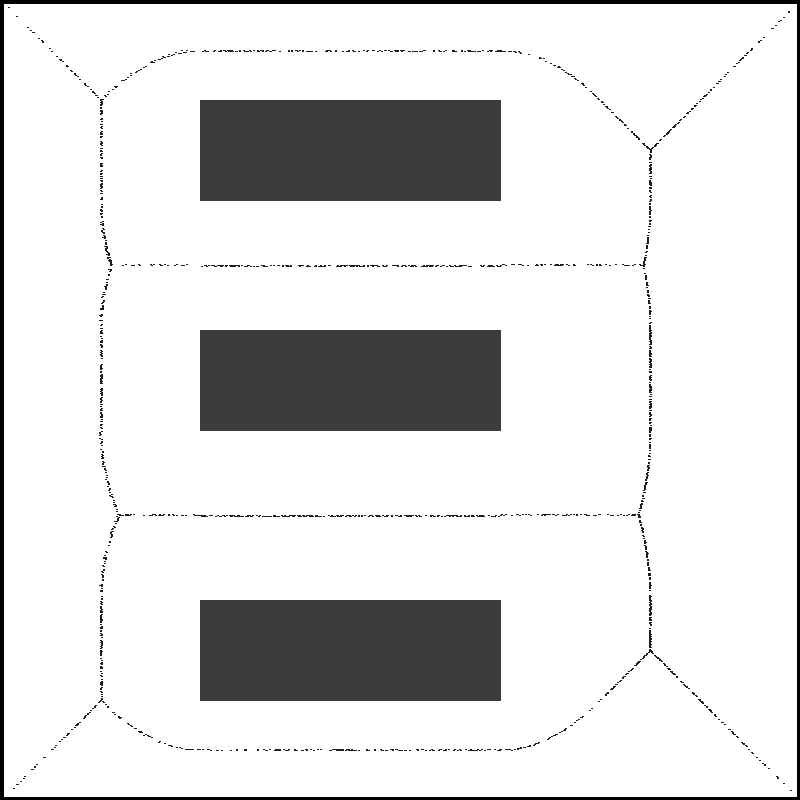
\includegraphics[scale=0.35]{./pics/MA.PNG}}
	\caption{\label{fig:Medial Axis} Sampling on the Medial Axis of a rectangle space. The black blocks are obstacles. We will use this world as our working space in the following sections. }
\end{figure}

%====================================
% Dual shapes of unions of balls
%====================================

\paragraph{C} \emph{Dual Shapes of Unions of Balls} \hfill\\
\indent Approximating the shape of an unknown area to study its properties is a very commonly used method. We have seen research ideas in the study of biogeometry to solve the problem. As for robotics, a few people began to notice the achievements from biogeometry study and tried to apply similar methods to study the shape of \emph{C-space}. \cite{alpha intro} 

\indent We have seen papers concerning the shape of \emph{C-space}. Robin, et al, developed a computational method for detecting large convex regions of obstacle-free space\cite{largeconvex}. Knowing such information can be helpful to plan robot footstep locations while avoiding obstacles and other optimization problems. But this method can only capture local features.

\indent Z. McCarthy, et al, \cite{PathNonexistance} used samples generated by PRM to form the $\alpha$-shape of \emph{C-space}. She then proved there doesn't exist a path between a pair of configurations by proving they are in two different disconnected components of the shape. She declared it was the first time $\alpha$-shape is being used in motion planning.

\indent Define a \emph{simplicial complex} $D$: a collection of simplices such that if $\bigtriangleup_T \subseteq D$ ( $\bigtriangleup_T$ is the convex hull of $T$ ), then if $U \subseteq T$, we have $\bigtriangleup_U \subseteq D$ and also that the intersection of two simplices in $D$ is either empty or another simplex in $D$. The $\alpha$-shape of a set of points $S$ is a generalization of the convex hull of those points\cite{PathNonexistance}. H. Edelsbrunner first introduced them in \cite{PointSetShape}. By choosing different values of the one parameter $\alpha$, we can have a family of shapes with the same set of points. An example of $\alpha$-shape is in Figure \ref{fig:Alpha-shape}.

\indent Choosing the best $\alpha$ value could be a bothering work. Assuming weighted points in the point set, by using a generalization of the Delaunay Triangulation, the Regular Triangulation, we can construct another shape using weights as flexible $\alpha$'s. Points with weights can be considered as balls. H. Edelsbrunner gave us this idea in \cite{DualShape}. Such shapes are also called Dual Shapes or Dual complex of unions of balls. The weighted $\alpha$-shape captures the topology of the union of balls with different radii. Figure \ref{fig:Dual Shape} shows an example of such weighted $\alpha$-shape.

\begin{figure}
	\center{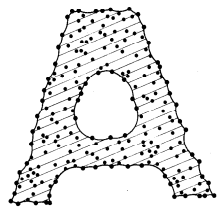
\includegraphics[scale=0.7]{./pics/alphaShape.png}}
	\caption{\label{fig:Alpha-shape} An example of $\alpha$-shape}
\end{figure}

\begin{figure}
	\center{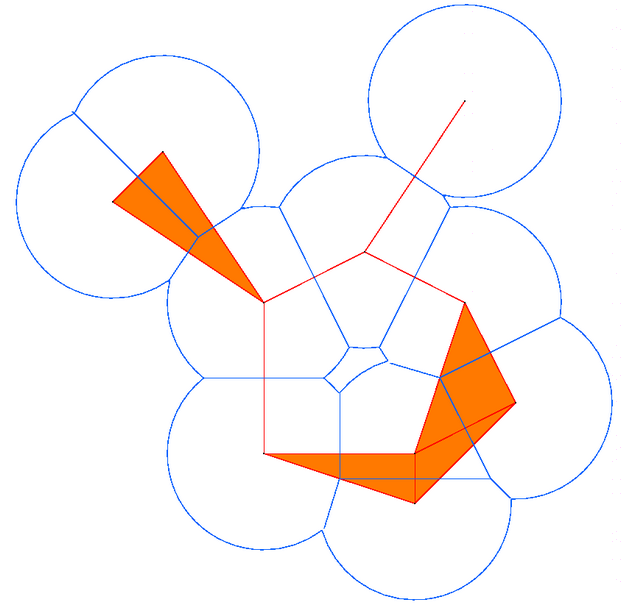
\includegraphics[scale=0.30]{./pics/dualshape.png}}
	\caption{\label{fig:Dual Shape} An example of weighted $\alpha$-shape for a union of balls. Copied from \cite{DualShape}}
\end{figure}

%====================================
% Betti Numbers
%====================================
\paragraph{D} \emph{Betti Numbers} \hfill \\
\indent In algebraic topology, the Betti Numbers are used to distinguish topological spaces based on the connectivity of n-dimensional simplicial complexes. Informally, the \emph{n-th} Betti number ($\beta_n$) represents the rank of the \emph{n-th} homology group, which tells us the maximum number of cuts that can be made before diving a surface into two pieces. \cite{betti wiki}

\indent An example of Betti numbers will be a torus. Figure \ref{fig:Torus}

\indent The first Betti number of a graph is very easy to compute. Given a graph $G$, with $n$ vertices, $m$ edges and $k$ components. It's 1st Betti number is

\begin{equation}
\beta_1 = m - n + k
\end{equation}

\indent Proof of this equation can be found in \cite{cyclomatic}.

\indent H. Edelsbrunner introduced a way to compute \emph{n-th} Betti number in \cite{Edel Book}, where he uses gaussian elimination to compute the Betti numbers with adjacency matrix.

\indent V. Robins \cite{alpha betti} provided a computational technique for computing Betti numbers with detailed explains and proofs. What's more, she put more thoughts on computing Betti numbers for alpha shapes.

\begin{figure}
	\center{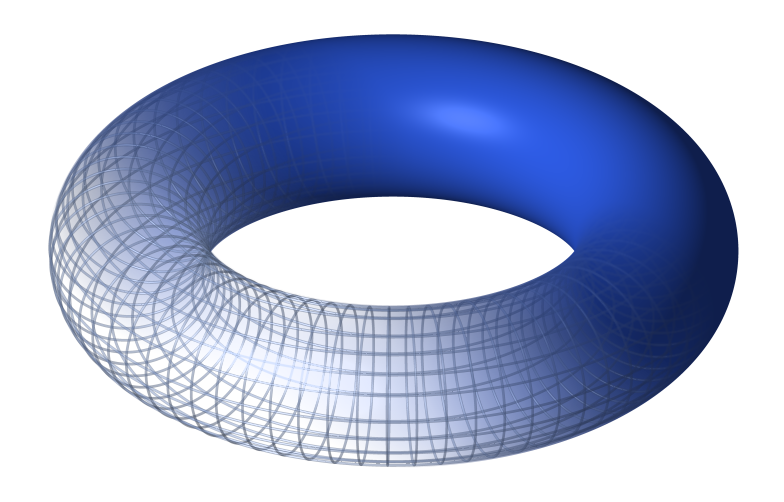
\includegraphics[scale=0.26]{./pics/Torus.png}}
	\caption{\label{fig:Torus} The torus has one connected component($\beta_0$), two circular holes ($\beta_1$,the one in the center and the one in the middle of the "donut"), and one two-dimensional void ($\beta_2$, the inside of the "donut"). Copied from \cite{betti wiki}}
\end{figure}


%%%%%%%%%%%%%%%%%%%%%%%%%%%%%%%%%%%%%%%%%%%%%%%%%%%%%%%%%%%%%%%%
%	Introduction to Our Algorithm
%
%%%%%%%%%%%%%%%%%%%%%%%%%%%%%%%%%%%%%%%%%%%%%%%%%%%%%%%%%%%%%%%%

\section{Our Method}\label{method} 

\indent \indent Traditionally, sampling based algorithms will build a graph for configuration space. Some of these graphs, such as \emph{PRM*} and \emph{RRT*} \cite{prmstar}, are proved to be able to find near optimal path, but can hardly be used to analysis the topology of paths. We want to to build a stronger representation of \emph{C-space} that is both able to cover optimal path and study the topological structure. In this section, we are trying to solve the problem in 2D and answer the question "Is two paths in the same homotopy class" as a start point of using our method to study the topology of \emph{C-space}. In this section, we will first give the outline of the algorithm, and explain each step in detail. 

\indent In the rest of the section, we will use the term "configuration" to refer to a point in configurations space.  Ball $B(x, \rho(x))$ is referred to as a $"sample"$ in the rest of the section. 

%====================================
% Algorithm outline
%====================================
\paragraph{A} \emph{The Algorithm outline} \hfill \\

\indent The algorithm is shown in Figure \ref{fig:Algo}. It has four phases. The first phase is to generate some random configurations in \emph{C-space}, like all other sampling-based planning algorithms do, and keep only those feasible ones. Every feasible configuration will be kept until the third phase. ($randomConfig$ keep unchanged.) In the second phase, we will sample balls centered on medial axis first and then try to cover the left area of $C_{free}$. Samples on the medial axis $MA(C_{free})$ will be used in phase three to construct the dual shape that captures the topology of $C_{free}$. After simplifying the dual shape, we will have a roadmap while maintaining the topological structure. Phase four breaks the topology roadmap into pieces such that no two piece can be merged into a new graph without forming a loop. 

\indent We will now explain each phase in detail with demos.

%%%%%%%%%%%%%%%%================================================>>>>>>>>>>>>>>>>>>>>>>>>>>>>>>
%%%%%%  We need to name our algorithm
%%%%%%  Seriously
%---------------------------------------------------------------------------------------------
\begin{figure}
  \begin{algorithmic}[1]
  \Function{RichCspaceRepresent}{\emph{C-space}, number}
  
    // Phase One
    \indent \State $randomConfigs \gets SampleRandomConfigurations( \emph{C-space}, number )$ 

    // Phase Two
    \indent \State $maSamples \gets SampleOnMedialAxis( randomConfigs )$
    \indent \State $regSamples \gets SampleLeftArea(maSamples, randomConfigs)$

    // Phase Three
    \indent \State $dualShape \gets WeightedAlphaShape( maSmaples )$
    \indent \State $topologyRoadmap \gets Retract(dualShape)$ 

    // Phase Four
    \indent \State $brokenRoads \gets BreakGraph( topologyRoadmap )$
    
    \indent 
	
  \EndFunction
  \end{algorithmic}
  \caption{\label{fig:Algo} Algorithm Outline. \emph{C-space} here means the metric space $(X, \rho)$ where we can know if a configuration is feasible and its clearance to nearest obstacles.}
\end{figure}

%====================================
% Covering C-space
%====================================
\paragraph{B} \emph{Sampling in C-space} \hfill \\
\indent As pointed out in Figure \ref{fig:Algo}, this phase has two parts: Sampling on medial axis, and sampling the rest of free space. 

\indent Sampling on medial axis is well studied in \cite{MAPRM} and \cite{UMAPRM}. Besides the positions of configurations, we also keep the clearance of each configuration, thus have some balls, or samples. We also require that no new ball, when sampling, is allowed to be centered inside any existing ones. For details of the algorithms, please refer to these two papers. One thing worth our notice is that using only algorithm mentioned in \cite{MAPRM}, we can get good result in narrow corridor but are more likely to ignore large open area. While using only \cite{UMAPRM} method, we can cover large open area well, but more likely to produce disconnected balls in narrow corridors. Therefore, running both algorithms is highly recommended. 

\indent The reason we sample on medial axis first is that 1.these balls are maximal ones as the definition of medial axis suggests, thus may reduce the number of samples we get, and 2.medial axis $MA(C_{free})$ is a SDR of \emph{C-space}. \cite{MAPRM2}

\indent Figure \ref{SampleLeftArea} describes how we sample area not yet covered by balls centered on medial axis. The basic idea behind the algorithm is to keep sampling new balls on the boundary of existing ones by "pushing" random configurations inside existing balls to the boundary of them and determine if they are in any other balls. If not, we sample a new ball. We restrict that all balls to be larger than a minimal radius ball, thus void getting a lot of very small samples.

\indent Getting configurations inside a ball doesn't have to be $O(n)$ costly. It can be done using KNN algorithm, which is more efficient than iterating everything. Since we generated random configurations $n$ times(not all are feasible), in a 2D space with area $A$. We expect to have $n/A$ configurations in an unit area. A ball with radius $r$ has area $\pi r^2$, approximately
\begin{equation}
k = n \cdot \pi r^2 / A
\end{equation} 
configurations are inside the ball. We then project these (uniformly distributed) configurations to the boundary of the ball to sample new spheres. Actually, choosing a larger $k$ could be better: we virtually extend the radius of our discs, which results in a smaller density in arcs that are very close to obstacles than those far from obstacles. Samples got in this part are called \emph{regular samples}. 

\indent Figure \ref{Samples} is a result of this phase running in a rectangle \emph{C-space} with 3 obstacles in the middle. Gray balls are centered on medial axis, while green ones are not. Red points are ball centers.

\begin{figure}
\begin{algorithmic}[1] 
  \Function{SampleLeftArea}{ maSamples, randomConfigs }
  	\State $regSamples \gets EmptySet$ \Comment{Set of balls not on MA}
  	\State $newBall \gets$ True	\Comment{If we can get new balls}
  	\State $lastRoundBalls \gets maSamples$
  	\While{$newBall$}
  		\State $newBall \gets False$
		\State $bndConfigs \gets EmptySet$ \Comment{A set of ball boundary configs}  		
  		\For {$ball \in lastRoundBalls$}
  			\State $innerConfigs \gets KNearest(ball, randomConfigs)$; \Comment{KNN}
  			\State $bndConfigs.append( getBoundaryConfigs(ball, innerConfigs) )$
  		\EndFor
  		\State $lastRoundBalls \gets EmptySet$
  		\For{$config \in bndConfigs$}
  			\If{$config$ not inside any existing ball} \Comment{ $O(n^2)$ time}
  				\State $ball \gets getNewBall(config)$ \Comment{get a new ball}
  				\If{$ball.radius \geq min\_radius$}
  					\State $newBall \gets True$
  					\State $lastRoundBalls.append( ball )$
  					\State $regSamples.append(ball);$
  				\EndIf
  			\EndIf
  		\EndFor
  	\EndWhile
  	\State \Return $regSamples$
  \EndFunction
  \end{algorithmic}
  \caption{\label{SampleLeftArea} Algorithm to sample left free area}
\end{figure}

\begin{figure}
	\center{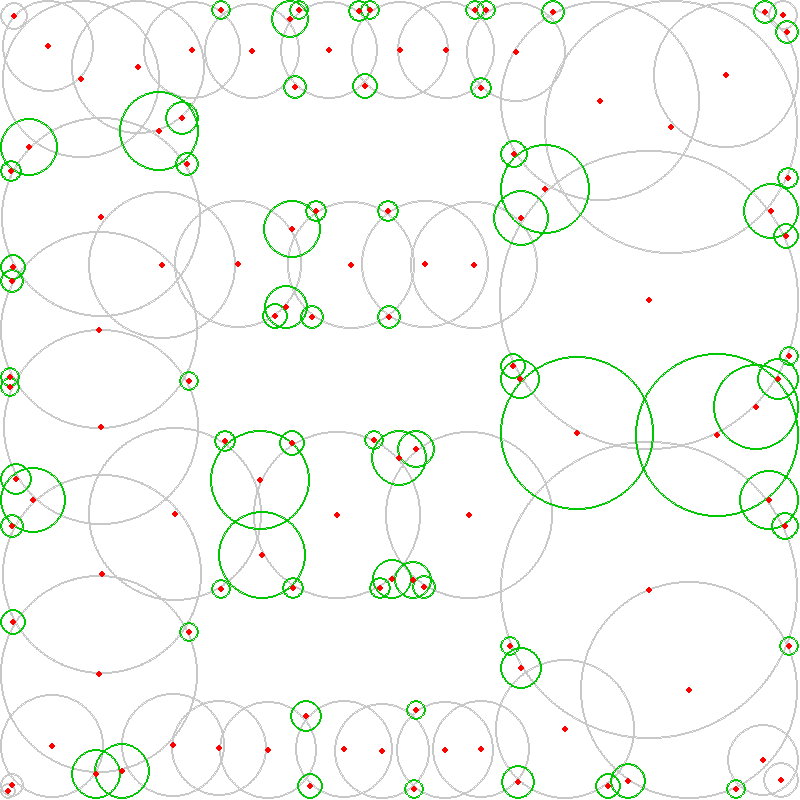
\includegraphics[scale=0.3]{./pics/Samples.PNG}}
	\caption{\label{Samples} Samples got by the algorithm}
\end{figure}

%====================================
% Dual shape and topology roadmap
%====================================

\paragraph{C} \emph{Constructing Topology Roadmap of C-space} \hfill \\
\indent After getting these samples, we can now start to build a structure that captures the topology of the space. 

\indent This phase, like the previous one, has two parts: 1. Construct the dual shape of medial axis samples got from phase one. 2. Simplify the dual shape to a simple graph.

\indent In the first part, constructing the dual shape using only the medial axis sample could break the topology of medial axis. The reason is shown in Figure \ref{badthing}: three balls are all centered on medial axis, but their dual shape will be an empty triangle, which introduces a "hole" in that area. To solve this problem we can try to sample a ball centered at the radical center after getting an empty triangle, and rebuild the dual shape for these four balls\cite{radical center}. A simple proof: if there is no obstacles in that area, the newly sampled ball will connect three balls, if there is obstacle, the ball will either not be sampled or not connect three of the balls.

\indent With these balls, we then compute their dual shape, which is formed by some 1-simplices and 2-simplices in 2D. The runtime of computing dual shape will be $O(n^2)$ which is the worst case when doing regular triangulation of weighted points. Although using all balls will avoid problem as in Figure \ref{badthing}, we are making $n$ much larger, which results in a bad runtime of this step. (However, constructing the dual shape of all balls will be helpful to study the shape of \emph{C-space})

\indent One might argue that we can simply get configurations on medial axis and connect them as a roadmap. However, this roadmap doesn't maintain the topology of \emph{C-space}. At some corners, we will still get triangles which don't have information if there are obstacles inside the triangle. By building the dual shape, this will no longer be a problem. 

\indent The second part of this phase can be stated as: retract all connected 2-simplices into one point, reconnect these retracted points with other ones using their previous connection. By doing so, we got a simple graph that characterize the topology of \emph{C-space}. We would like to call it \emph{Topology Roadmap}. This roadmap can also be used to determine if paths exist between two configurations. An example of such roadmap is shown in Figure \ref{simplifiedgraph}. Filled triangles, along with large balls, are suggesting some large open areas, which is a problem \cite{largeconvex} is trying to address. 

\indent This is not the only method of building the topology roadmap of \emph{C-space}, another option will be to build a visibility roadmap, like \cite{vprm}, but using only ball centers as roadmap nodes. One might come up with other heuristics to achieve the same thing. Due to the limited number of balls, any algorithms can have a good performance. 

\indent 

\begin{figure}
	\center{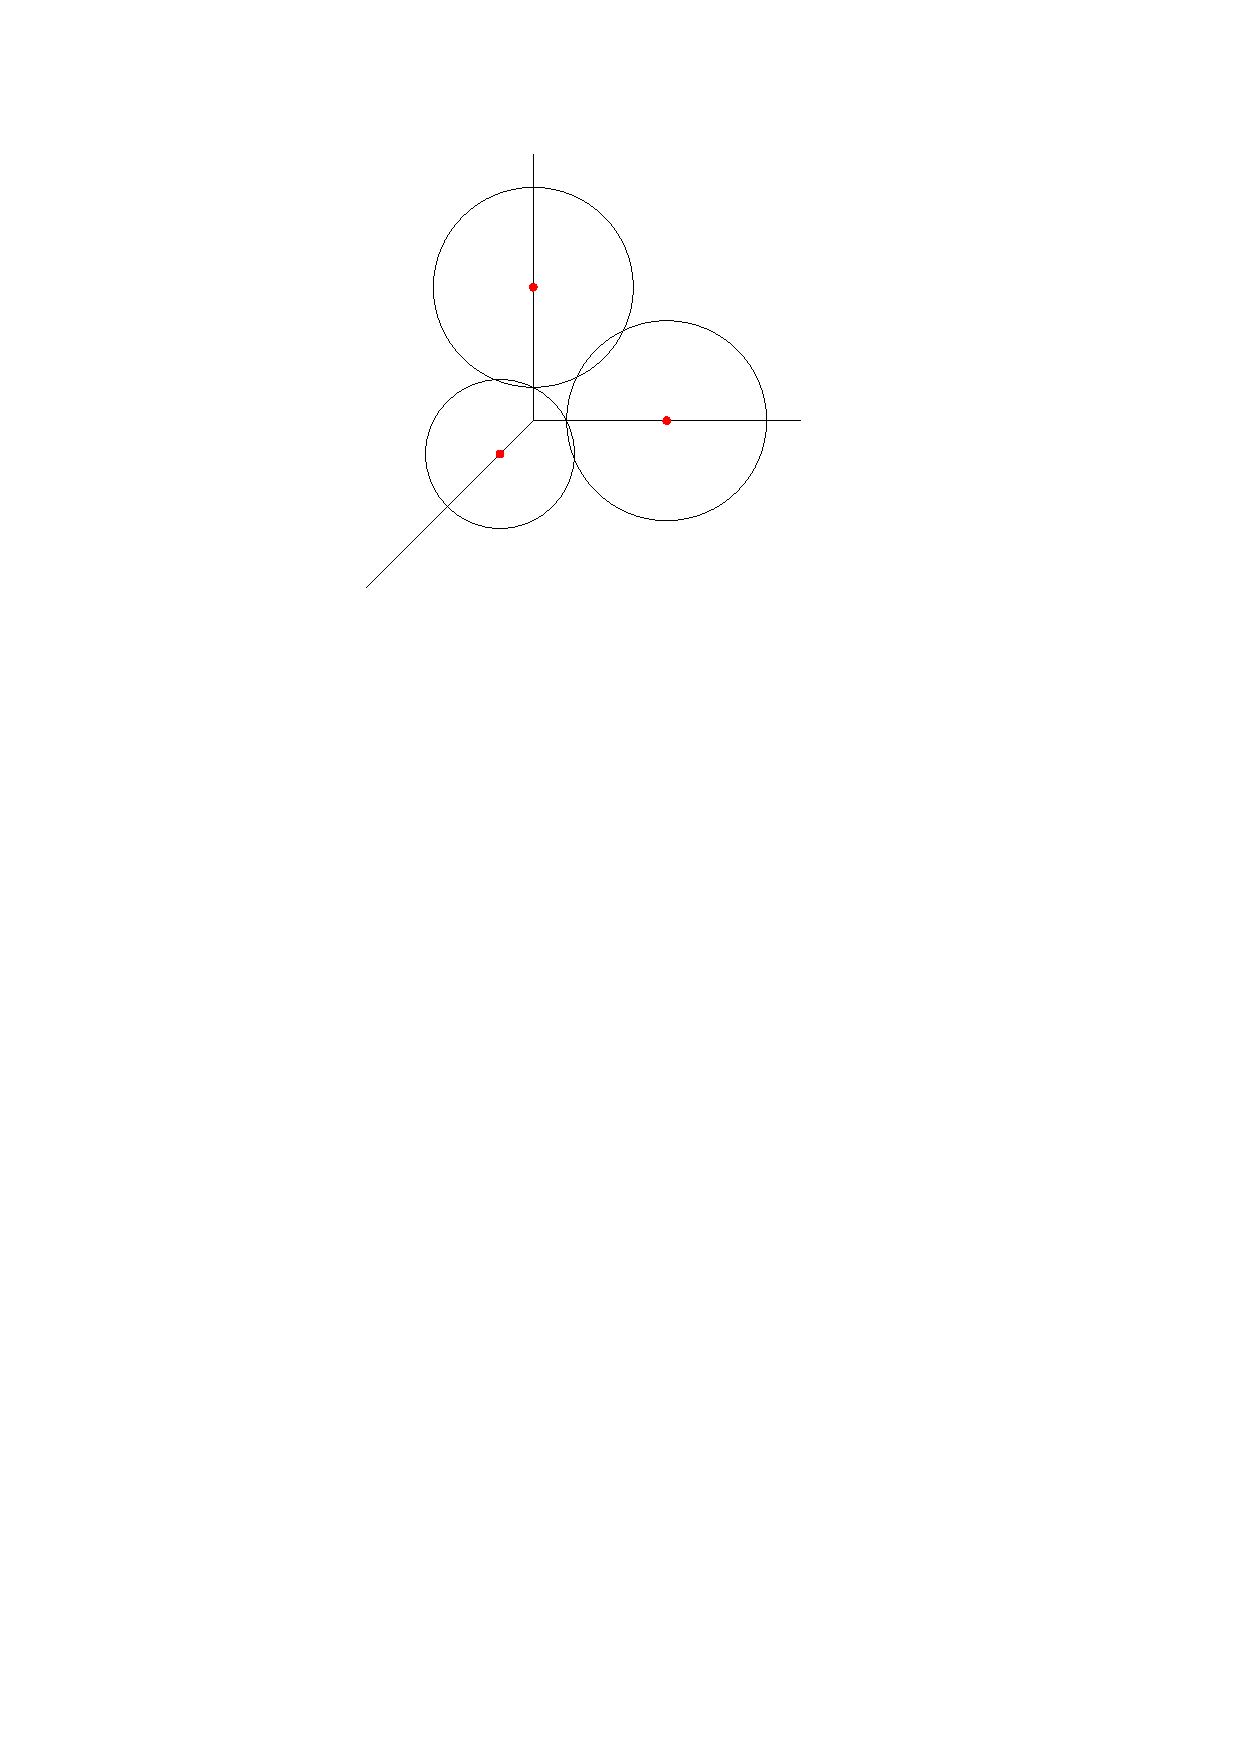
\includegraphics[scale=1]{./pics/badthing.pdf}}
	\caption{\label{badthing}} An example that medial axis samples break the topology structure of the medial axis.
\end{figure}

\begin{figure}
	\center{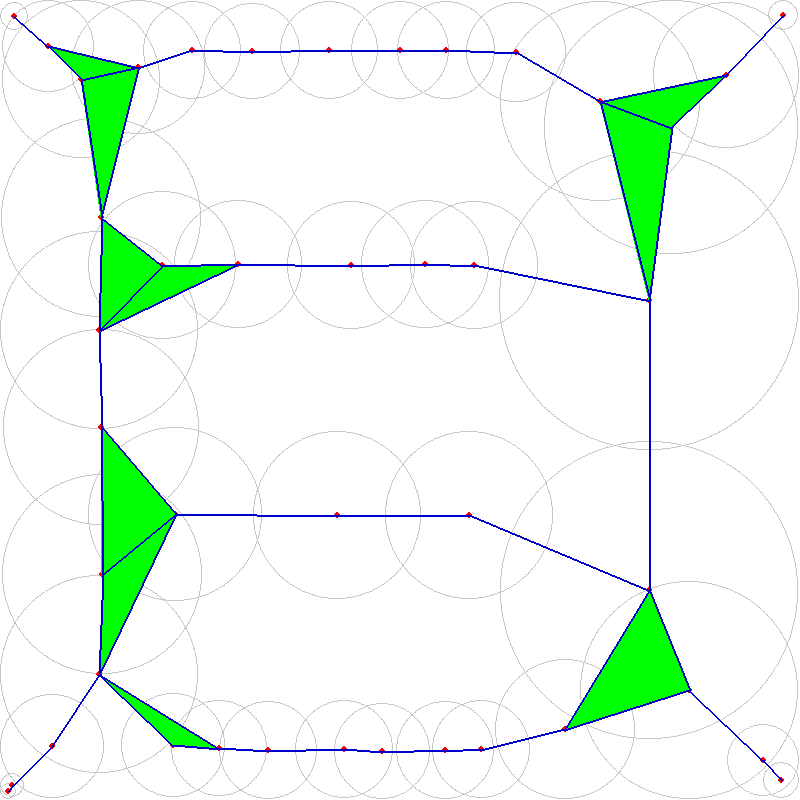
\includegraphics[scale=0.3]{./pics/my_dualshape.PNG}}
	\caption{\label{ourdualshape}} Dual shape of balls generated in phase 1 (centered on medial axis). Filled triangles, along with large balls, are suggesting some large open areas.  
\end{figure}

\begin{figure}
	\center{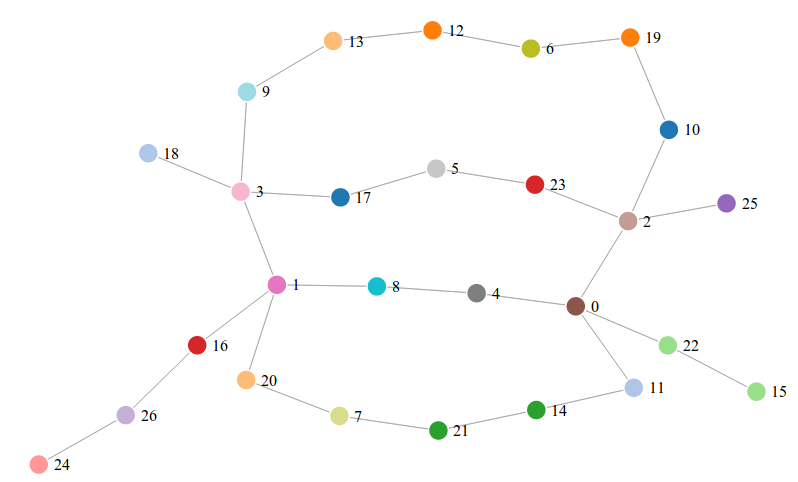
\includegraphics[scale=0.4]{./pics/simplified_graph.png}}
	\caption{\label{simplifiedgraph}} Simplified graph of the dual shape in Figure \ref{ourdualshape}.
\end{figure}

%====================================
% Break graph
%====================================
\paragraph{D} \emph{Breaking A Graph into Loop-free Parts} \hfill\\
\indent After getting the topology roadmap, we technically already have a planner, but still we can simplify it. We now discuss breaking a graph into several components, such that no two components can merge into a new graph without forming a loop. By doing this, a graph is even simplified. Knowing which components are the start and goal configurations in, we can find a path connecting these components immediately. This technique can be a great improve when \emph{C-space} is very large and traditional \emph{PRM} or \emph{RRT} methods will take a long time to solve.

\indent Let $g_1$ and $g_2$ be two graphs without loops. We say $g_1$ and $g_2$ to be \emph{mergeable} if: 1. they share at least one common node, 2. the new graph formed by these two graph has no loop. 

\indent Determine if a simple graph has a loop is very easy using the first Betti number $\beta_1$ mentioned in section 2, equation (1). 

\indent Figure \ref{breakgraph} shows our algorithm to break a graph. The idea behind this algorithm is to take every edges as an initial component, then iterate each component to find and merge with a mergeable component until there is no two mergeable components.

\indent By breaking a graph into several parts, we virtually break the space into several subspaces. In this sense, our method can be viewed as a space partition strategy.

\begin{figure}
\begin{algorithmic}[1] 
  \Function{BreakGraph}{ graph }
  	\State $components \gets EmptySet$
  	\For {$edge \in graph.edges$}
  		\State components.append( new Graph(edge) )
  	\EndFor
  	
  	\State \Return MergeComponents( components )
  \EndFunction
\end{algorithmic}


\begin{algorithmic}[1]   
  \Function{MergeComponents}{components}
  	\State $pq \gets PriorityQueue()$
    \For{$component \in components$}
        \State $pq.push(component, component.size())$
    \EndFor
    \While{ $pq.size() > 1$ }
    	\State $smallest\_component \gets pq.pop()$
    	\State $mergeable\_component \gets$ \emph{find first mergeable component in pq}
		\State $new\_component \gets smallest\_component.merge\_with( mergeable\_component )$
    	\State $components.remove( smallest\_component )$
    	\State $components.remove( mergeable\_component )$
    	\State $pq.remove( mergeable\_component )$
    	\State $components.append( new\_component )$
    	\State $pq.push(new\_component, new\_component.size())$
	\EndWhile
	
    \State \Return $components$
  \EndFunction  
\end{algorithmic}
	\caption{\label{breakgraph}} Breaking a graph into several loop-free components.
\end{figure}

\begin{figure}
	{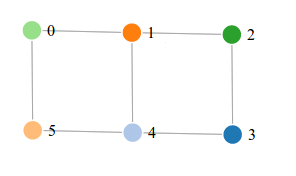
\includegraphics[scale=0.7]{./pics/initial.png}}
	{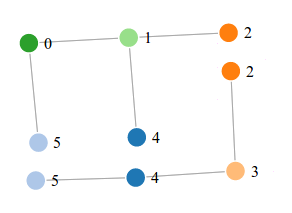
\includegraphics[scale=0.7]{./pics/broken.png}}
	
	{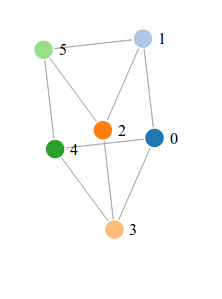
\includegraphics[scale=0.65]{./pics/initial2.png}}
	{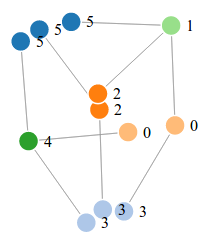
\includegraphics[scale=0.65]{./pics/broken2.png}}\
	\caption{\label{brokengraphs} Some examples of breaking a graph. Graphs are visualized using $d3.js$ $(http://www.d3js.org)$ }
\end{figure}

%====================================
% Path topology
%====================================
\paragraph{E} \emph{Determine Paths in the Same Homotopy Class} \hfill \\
\indent A continuous function, or a map, $f: X \rightarrow Y$ is called a \emph{homotopy equivalence} if there is a map $g: X \rightarrow Y$ such that there exist a continuous function $H: X \times [0,1] \rightarrow Y$ with $H(x, 0) = f$ and $H(x,1) = g$.

\indent Besides using those components to plan motions for a large \emph{C-space}, they can also be used to determine if two paths are in the same homotopy class. 

\indent Let $\sigma_1$ and $\sigma_2$ be two paths, with the same start and goal configuration, going through from components $g_1$ to $g_2$ via two nodes $A$ and $B$. $\sigma_1$ and $\sigma_2$ are homotopy equivalent if $A = B$. 

\indent Proof can be found in section 4.

%%%%%%%%%%%%%%%%%%%%%%%%%%%%%%%%%%%%%%%%%%%%%%%%%%%%%%%%%%%%%%%%
%	Properties of Our Algorithm
%
%%%%%%%%%%%%%%%%%%%%%%%%%%%%%%%%%%%%%%%%%%%%%%%%%%%%%%%%%%%%%%%%
\section{Good Properties}\label{properties}
\indent\indent This section should be re-organized as below:
  \subsection{Coverage Analysis}
  \begin{theorem}
  Let $S_{init}$ be the set of initial random configurations. With minimum radius of $r_{min}$, configurations with clearance larger than $r_{min}$ will be covered, when $|S_{init}| \rightarrow \infty$.
  \end{theorem}
    
  \paragraph{\emph{Proof:}} 
  \indent When the number of initial random configurations approaches infinite, the boundaries of all existing balls are fully covered. So, every configuration not inside any existing balls will be sampled as a ball, unless it's less than $r_{min}$ clearance.\\
  
  As we can see, we can analyze the coverage of the space. Even more, we can explicitly describe the coverage of each ball in the algorithm. Using this property, we can find near optimal path. We will show some experiments in section 5.
  
  \begin{theorem}
  Let $b \in B$ be an element of $B$, $A$ and $B$ are two configurations in \emph{C-space}. The optimal path $\sigma$ between $A$ and $B$ is in $\bigcup_{b\in B}$ if $\sigma$ has clearance no less than $r_min$. 
  \end{theorem}   
  \paragraph{\emph{Proof}}
  \indent This is a direct conclusion of previous theorem.

  \subsection{Low Memory Representation}  
  \begin{theorem}
  Let $B$ be the set of ball samples got in phase one. Then $|B|$ is finite.   
  \end{theorem}
  \paragraph{\emph{Proof:}} 
  \indent We restrict balls to have no less than $r_{min}$ radius and new balls to be centered outside existing ones. Assume we partition the space into $r_{min} \times r_{min}$ cells in 2D. The number of cells is finite, if the space is finite. Putting balls with exactly $r_{min}$ radius in the centers of these cells will cover the space totally. The number of balls is finite. Phase one will generate balls no more than the number of balls generated in this way. Figure \ref{ourdualshape} shows the dual shape of balls generated by previous phase.  \\
  
  In practice, most balls are much larger than minimum radius. So the actually number of balls is very limited. We will see, in section 5, the number of balls required to cover a space tends to be stable. 
  
  \subsection{Analysis of Topology}
  
  In this subsection, we will see how to use the structure built by our algorithm to determine path topology.  
      
  \begin{theorem}
  Any path $\sigma$ can be continuously deformed onto medial axis. 
  \end{theorem}   
  \paragraph{\emph{Proof}}
  \indent This is the definition of Medial Axis $MA(C_{free})$ being a strong deformation retraction of $C_{free}$.\\
  
  Given the theorem that any path can be deformed onto medial axis, we now use medial axis samples to determine if two paths have the same homotopy type.
  
  \begin{theorem}
  Given path $\sigma_1$ and $\sigma_2$, we say they have the same homotopy type if their image in the topology roadmap is the same. 
  \end{theorem}
  \paragraph{\emph{Proof}}
  \indent Let $x$ be a point in the space $X$, $B = \{ b_1, b_2, ..., b_n \}$ be the set of balls centered on medial axis. Define map $H(x)$:
  \begin{equation}
  H(x) = b_i \indent, if \indent |x-b| \leq |x-b'|, b' \in B
  \end{equation}
  \indent This continuous function maps any points in the space to balls centered on medial axis. While every point in the balls is mapped to the dual shape form by filled triangles, nodes and edges. Filled triangles are mapped to single nodes.   
  
  \indent Therefore, if two paths have the same image in the topology roadmap. They have the same homotopy type.

%  \begin{theorem}
%  Let $g_1$ and $g_2$ be two loop-free graphs such that merging their common nodes will produce a new graph with loops. Let $\sigma_1$ and $\sigma_2$, with the same start and goal nodes, be two paths going from $g_1$ to $g_2$ via common nodes $A$ and $B$. $\sigma_1$ and $\sigma_2$ have different homotopy type if $A \neq B$
%  \end{theorem}
%  \paragraph{\emph{Proof}}
%  \indent Let start and goal nodes be $S$ and $E$. Because $A$ and $B$ are two common nodes shared by $g_1$ and $g_2$, if $A \neq B$, merging $g_1$ and $g_2$ will create a graph with a loop going from $S \rightarrow A \rightarrow E \rightarrow B \rightarrow S$. The path in the upper of the loop and the path in the lower have different homotopy type. Since $\sigma_1$ and $\sigma_2$ have the same start and goal nodes, merging them will create a loop. So $\sigma_1$ and $\sigma_2$ have different homotopy type.

  \subsection{Fast Planning}
  \indent\indent By breaking a graph into several parts, we virtually break the space into several subspaces. In this sense, our method can be viewed as a space partition strategy. Every subspace is managed by a tree, and trees are connected with shared common nodes. Every node in a tree represents a cell of power-diagram, as suggested by equation (3).
  
  \indent 
  

%%%%%%%%%%%%%%%%%%%%%%%%%%%%%%%%%%%%%%%%%%%%%%%%%%%%%%%%%%%%%%%%
%	Experiments
%
%%%%%%%%%%%%%%%%%%%%%%%%%%%%%%%%%%%%%%%%%%%%%%%%%%%%%%%%%%%%%%%%
\section{Experiments}\label{experiments}
We now describe the some experiments and their results.

%%%%%%%%%%%%%%%%%%%%%%%%%%%%%%%%%%%%%%%%%%%%%%%%%%%%%%%%%%%%%%%%
%	Conclusions and Future work
%
%%%%%%%%%%%%%%%%%%%%%%%%%%%%%%%%%%%%%%%%%%%%%%%%%%%%%%%%%%%%%%%%
\section{Conclusions and Future Work}\label{conclusions}
\indent\indent The results demonstrated with our algorithm are sound for covering the \emph{C-space} and represent the topology.  

\indent However, we don't know what kind of issues there will be when implementing for high dimensional space. The time cost for constructing weighted $\alpha$-shape( dual shape ) of unions of balls is a concern. Because we need to check each \emph{k-simplex} while $k = 1, 2, 3, ..., d$, $d$ being the dimensions. So, our next goal is to implement the algorithm for 3D case, and then higher dimensions.

\indent Our next direction is to study the properties and applications of weighted $\alpha$-shape, especially applications in bioinformatics and chemistry, then extend to high dimensions.

\indent Another direction will be studying the topology using the topology roadmap we constructed. Its value is underestimated in this paper, and I believe we can find more there.

\bibliographystyle{abbrv}
\begin{thebibliography}{1}
  \bibitem{weifu} Weifu Wang, Devin Balkcom, Amit Chakrabarti, ``A fast streaming spanner algorithm for incrementally constructing sparse roadmaps", IROS 2013.
  \bibitem{bekris} Marble J and Bekris KE. ``Asymptotically near-optimal planning with probabilistic roadmap spanners", IEEE Transactions on Robotics, 29(3), 2013.
  \bibitem{largeconvex} Robin L H Deits and Russ Tedrake. ``Computing large convex regions of obstacle-free space through semidefinite programming". In Proceedings of the Eleventh International Workshop on the Algorithmic Foundations of Robotics (WAFR 2014), Istanbul, 2014.
  \bibitem{sampissues} Lindemann, Stephen R., and Steven M. LaValle. ``Current issues in sampling-based motion planning." Robotics Research. Springer Berlin Heidelberg, 2005. 36-54.
  \bibitem{pathtopsearch} Bhattacharya, Subhrajit, Maxim Likhachev, and Vijay Kumar. ``Topological constraints in search-based robot path planning." Autonomous Robots 33.3 (2012): 273-290.
  \bibitem{pathtop} Bhattacharya, Subhrajit, Vijay Kumar, and Maxim Likhachev. ``Search-based path planning with homotopy class constraints." Third Annual Symposium on Combinatorial Search. 2010.
  \bibitem{prmstar} Sertac Karaman, Emilio Frazzoli, ``Sampling-based Algorithms for Optimal Motion Planning", International Journal of Robotic Research - IJRR , vol. abs/1105.1, no. 7, pp. 846-894, 2011.
  \bibitem{vprm} Thierry Siméon, Jean-paul Laumond, Carole Nissoux, ``Visibility-based probabilistic roadmaps for motion planning", Advanced Robotics , vol. 14, no. 6, pp. 477-493, 2000.
  \bibitem{aug} J.-M. Lien, O. B. Bayazit, R.-T. Sowell, S. Rodriguez, and N. M. Amato. ``Shepherding behaviors". In Proc. IEEE Int. Conf. Robot.Autom. (ICRA), pages 4159–4164, April 2004.
  \bibitem{design} O. B. Bayazit, G. Song, and N. M. Amato. ``Enhancing randomized motion planners: Exploring with haptic hints". In Proc. IEEE Int. Conf. Robot. Autom. (ICRA), pages 529–536, 2000.
  \bibitem{bioinformatics} A. P. Singh, J.-C. Latombe, and D. L. Brutlag. ``A motion planning approach to flexible ligand binding". In Int. Conf. on Intelligent Systems for Molecular Biology (ISMB), pages 252–261, 1999.
  \bibitem{ConCompNum} Delanoue, N.; Jaulin, L.; Cottenceau, B. (2006). ``Counting the Number of Connected Components of a Set and Its Application to Robotics". Applied Parallel Computing, Lecture Notes in Computer Science 3732 (1).
  \bibitem{interval} Jaulin, L. (2001). ``Path planning using intervals and graphs". Reliable Computing 7 (1).  
  \bibitem{Book} Steven M. LaValle, ``Planning Algorithms", Cambridge University Press, ISBN 0-521-86205-1, 2006.
  \bibitem{UMAPRM} Yeh, Hsin-Yi Cindy, et al. ``UMAPRM: Uniformly Sampling the Medial Axis."
  \bibitem{RRT} LaValle, Steven M. ``Rapidly-Exploring Random Trees A New Tool for Path Planning." (1998).
  \bibitem{PRM} L. E. Kavraki, P. Svestka, L. E. K. P. Vestka, J. claude Latombe, and M. H. Overmars, ``Probabilistic roadmaps for path planning in high-dimensional configuration spaces" IEEE Trans. Robot. Autom., vol. 12, pp. 566–580, 1996.
  \bibitem{MAPRM} Wilmarth, Steven A., Nancy M. Amato, and Peter F. Stiller. ``MAPRM: A probabilistic roadmap planner with sampling on the medial axis of the free space." Robotics and Automation, 1999. Proceedings. 1999 IEEE International Conference on. Vol. 2. IEEE, 1999.
  \bibitem{MAPRM2} S. A. Wilmarth, N. M. Amato, and P. F. Stiller. ``MAPRM: A probabilistic roadmap planner with sampling on the medial axis of the free space". Technical Report TR98-022, Department of Computer Science, Texas A\&M University, College Station, TX, Nov. 1998.
  \bibitem{DualShape} Edelsbrunner, Herbert. ``The union of balls and its dual shape." Proceedings of the ninth annual symposium on Computational geometry. ACM, 1993.
  \bibitem{alpha intro} ``Alpha Shape Introduction", Duck University, ($http://biogeometry.duke.edu/software/alphashapes/$)
  \bibitem{PointSetShape} Edelsbrunner, Herbert; Kirkpatrick, David G.; Seidel, Raimund (1983), ``On the shape of a set of points in the plane", IEEE Transactions on Information Theory 29 (4): 551–559, doi:10.1109/TIT.1983.1056714.
  \bibitem{radical center} ``Radical Center", From Wolfram MathWorld -- the web's most extensive mathematics resource. ($http://mathworld.wolfram.com/RadicalCenter.html$)
  \bibitem{PathNonexistance} Z. McCarthy. Bretl, and S. Hutchinson, ``Proving path non-existence using sampling and alpha shapes," in IEEE International Conference on Robotics and Automation (ICRA), May 2012.
  \bibitem{betti wiki} ``Betti Number", From Wikipedia -- The Free Encyclopedia. ( $http://en.wikipedia.org/wiki/Betti_number$ )   
  \bibitem{cyclomatic} GYULA KAROLYI, AMBRUS PAL, ``The cyclomatic number of connected graphs without solvable orbits", Periodica Mathematica Hungarica, 01/2007; 
  \bibitem{Edel Book}Edelsbrunner, Herbert, and John Harer. ``Computational topology: an introduction." American Mathematical Soc., 2010. page. 88 - 93.
  \bibitem{alpha betti} Robins, Vanessa. ``Computational topology for point data: Betti numbers of α-shapes." Morphology of Condensed Matter. Springer Berlin Heidelberg, 2002. 261-274.
\end{thebibliography}

\end{document}